\chapter{Service Function Chain Implementation} 
\label{chap:vnf_ns_impl}

The complexity behind the creation of a working Service Function Chain system
was high demanding for particular care and a separated study. Indeed, the SFCs
are the at the core of the whole architecture: packet transmission and
elaboration is made here. Challenges regarding this topic are building a system
that is flexible enough to allow dynamic packet routing, support scalability and
provide methods to recovery from failures. In this chapter, a brief explanation
about the challenges and the issues encountered building this system are given.

\section{Harbor}

As already cited, Harbor acts as a MANO, orchestrating and managing VNFs and the
related services. From the SFC point of view, it carries consistency checks when
a NS definition is created. The checks are carried out based on the VNF ID.
While the VNF definition corresponds to a YAML Kubernetes configuration, the NS
one is a JSON array, as illustrated in this example:

\begin{lstlisting}[caption={Example of SFC definition}, captionpos=b,
                   language=json, label=chap:impl:lst:sfcexample]
{
    "ns" : [
                {
                    "id": "astaire-service"
                },
                ...
            ]
}
\end{lstlisting}



\section{Kubernetes Pods}

All the SFC-related components have been developed with the idea of being
containerized. This is a fundamental concept, because in this way all the
components have the possibility to run inside Kubernetes, granting them the
scalability and persistence benefits. On top of that, the use of the Kubernetes
\verb!Deployment! feature granted the possibility to easily perform updates of
already existing components.

\section{Approved proposal}

\begin{figure}[t]
  \centering
  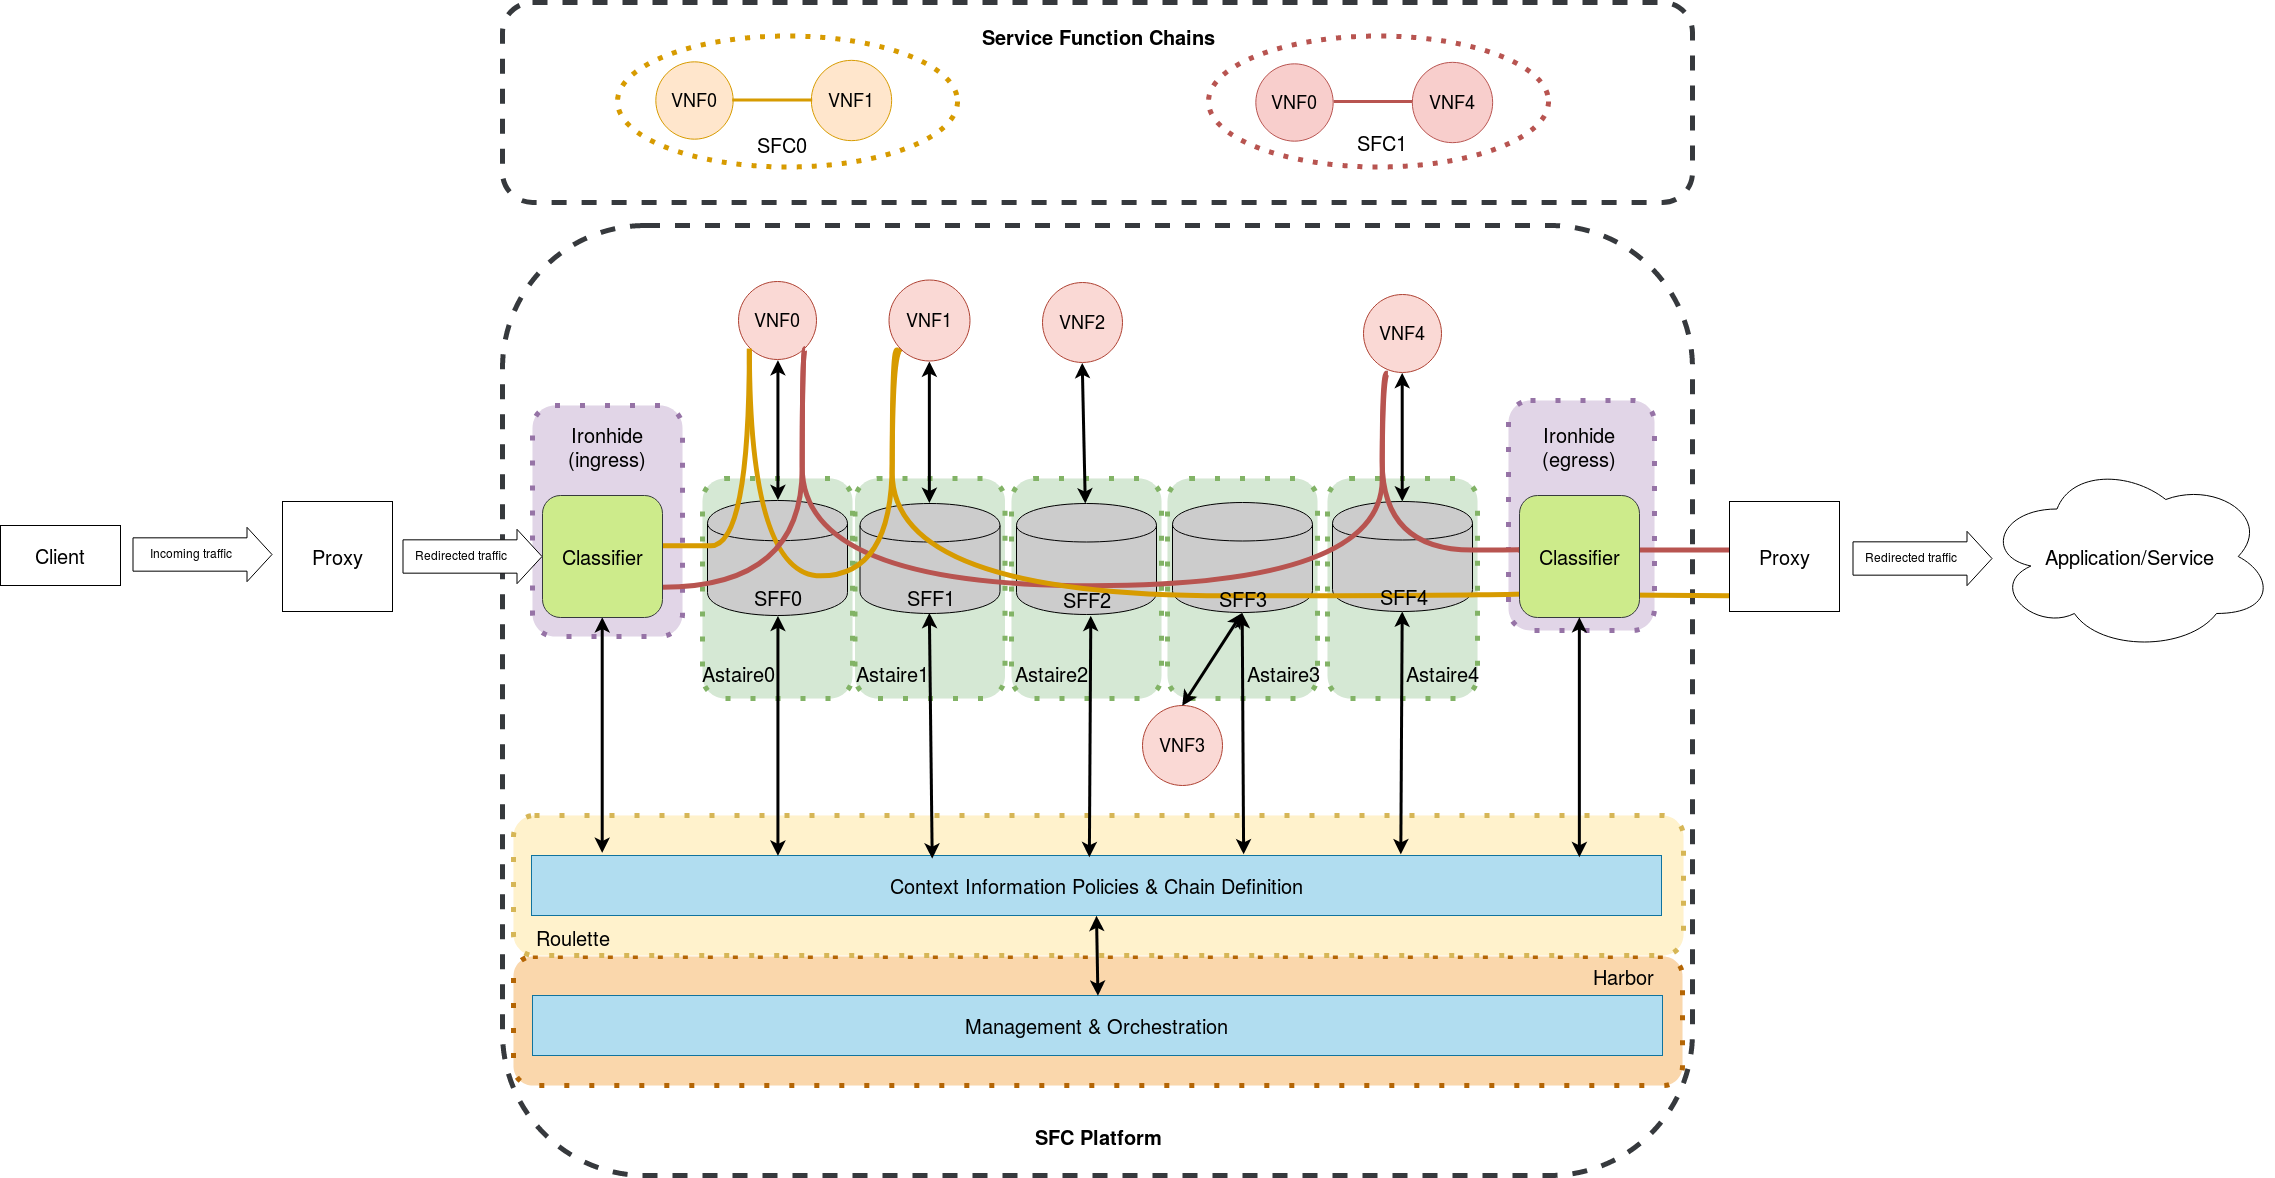
\includegraphics[width=\textwidth]{finalreview}
  \caption{Final review schema}
  \label{chap:impl:img:finalreview}
\end{figure}
In Figure~\ref{chap:impl:img:finalreview} is shown a high level schema
evidencing the components and their relationships. The approved proposal for the
creation of a proper chain has been based on four components:
\begin{itemize}
\item Astaire, which aim is to performing packet encapsulation and decapsulation
  between VNFs;
\item Harbor, which acts as our MANO component;
\item Ironhide, that provides ingress and egress point from our architecture;
\item Roulette, that stores endpoint information and holds the SFC topology
  view.
\end{itemize}

In this context our chain has the ability to perform packet classification,
making the whole system able to separate the traffic based on a packet-type
policy. 

Another important aspect to keep in consideration is how communications inside
the chain are performed. The packet arriving in the ingress needs to be
preserved, so that VNFs can perform packet elaboration. In order to obtain this,
packet encapsulation has been used. An IP/IP encapsulation allows to preserve
the original packet, making the incoming packet the payload of a new one.

Ironhide, which was introduced in the previous chapter, plays a crucial role in
the establishment of an end-to-end connection between the client and the
receiver. Ironhide is able to fulfill the ingress and the egress role, and it
provides the necessary tools to add and remove the SFC headers.

Finally, we were able to create bidirectional chains, resistant to faults and
degradations that satisfy the defined requirements.
